%Cosas Pendientes de Manuel Navarro García

\textbf{Número 1.1.} Sea $\mathcal{X}$ un conjunto, y $\T_{\text{CF}}$ la familia de todos los subconjuntos de $\mathcal{X}$ cuyo complementario es finito, más el conjunto vacío. Probar que $\T_{\text{CF}}$ es una topología en $X$. Esta topología se llama, por razones evidentes, \textit{topología de los complementarios finitos}. ?`Qué topología obtenemos si $\mathcal{X}$ es un conjunto finito?  \\

A partir del enunciado se deduce que los abiertos de esta topología son los elementos de la colección 

\[\T_{\text{CF}}= \{U \subset \mathcal{X} : U= \emptyset \text{ o } \mathcal{X} \backslash U\equiv U^c \text{ es finito}\}.\]

Veamos que efectivamente $\T_{\text{CF}}$ es una topología al verificar las condiciones necesarias. 

\begin{itemize}
\item En primer lugar, el vacío pertenece a esta por definición. Además, el complementario del total $\mathcal{X}$ (el vacío) es finito, luego $\mathcal{X}$ también pertenece a $\T_{\text{CF}}$. 

\item Por otro lado, sea $\{U_\alpha\}_{\alpha \in I}$ para un cierto conjunto de índices $I$ una colección arbitraria de elementos de $\T_{\text{CF}}$, teniéndose que 

\[\mathcal{X} \backslash \bigcup_{\alpha}U_\alpha = \bigcap_{\alpha} (\mathcal{X}\backslash U_\alpha).\]

Pero $\mathcal{X}-U_\alpha$ es finito para cada $\alpha \in I$, luego la intersección numerable de ellos también lo será. De este modo, la unión numerable de abiertos de $\T_{\text{CF}}$ pertenece a ella.

\item Por último, consideremos $U_1$ y $U_2$ dos abiertos de $\T_{\text{CF}}$. Analógamente al caso anterior, 

\[\mathcal{X} \backslash (U_1 \cap U_2) = \bigcup_{i=1}^2 (\mathcal{X}\backslash U_i).\]

Sin embargo, $\mathcal{X} \backslash U_i$ es finito para $i\in\{1,2\}$, luego la unión finita de conjuntos finitos es finita.
\end{itemize}

Para finalizar, se nos pregunta qué topología se obtendría en caso de que $\mathcal{X}$ fuese un conjunto finito. Si damos por cierta esta suposición, es claro que $\T_{\text{CF}}$ coincide con la topología discreta, ya que el complementario de todo conjunto es finito. \\

A pesar de haber terminado con lo requerido del ejercicio, podemos ir más allá estudiando más a fondo esta topología. Para comenzar, nótese que si $\mathcal{X}$ es numerable trivialmente el conjunto es separable y primer y segundo axioma de numerabilidad. El caso en el que $\mathcal{X}$ no es numerable ya no es tan sencillo. Vayamos por partes.

\begin{itemize}
\item $\mathcal{X}$ es separable. Es más, todo conjunto numerable es denso en $\mathcal{X}$. En efecto, supongamos que existiese un conjunto $A \subset \mathcal{X}$ numerable pero que no es denso en $\mathcal{X}$. Esto implica que existe un abierto $B\in \T_{\text{CF}}$ tal que $B\cap A = \emptyset$. De este modo, 

\[(\mathcal{X}\backslash B)\cup (\mathcal{X}\backslash A)=\mathcal{X}.\]

Pero los conjuntos del primer miembro son finitos, y la unión de finitos es finita, lo que conllevaría a que $\mathcal{X}$ también lo sea. Esto nos conduce a la  contradicción buscada. 

\item $\mathcal{X}$ no es primer axioma de numerabilidad, lo que implica que tampoco es segundo. Para corroborar esto, comprobemos que para cada punto $a\in \mathcal{X}$ no existe una base de entornos abiertos numerable centrada en $a$. Razonaremos de nuevo por reducción al absurdo.

Supongamos que sí que existe esa base y sea esta 

\[\mathcal{U}^a=\{V_k \in\T_{\text{CF}}: k \geq 1\}.\]

La intersección 

\[\left(\bigcap_{k\geq 1} V_k\right)\backslash \{a\}\]

es no vacía puesto que, al tomar los complementarios y aplicar las leyes de De Morgan se tiene que 

\[\mathcal{X} \backslash \left(\bigcap_{k\geq 1} V_k\right)= \left(\bigcup_{k\geq 1} \mathcal{X} \backslash V_k\right), \]

y esta unión es numerable ya que $X \backslash V_k$ es finito (recordemos que $V_k \in \T_{\text{CF}}$). Al ser $\mathcal{X}$ no numerable y 

\[\mathcal{X}= \left(\bigcap_{k\geq 1} V_k\right) \cup \left(\bigcup_{k\geq 1} \mathcal{X}\backslash V_k\right),\]

la intersección anterior ha de ser no numerable.

Tomemos ahora un punto cualquiera $b$ de esta intersección con la condición de que sea distinto de $a$ y consideremos el entorno abierto de $a$ dado por $W:=\mathcal{X}\backslash \{b\}$. Claramente, $a\in W$ y es abierto puesto que su complementario es finito.  De forma evidente la condición $V_k \subset W$ no se verifica para ningún $k$ ya que $b\in V_k$ para todo $k$. Esto verifica que $\mathcal{U}^a$ no puede ser base, concluyendo así que cuando $X$ no es numerable $\T_{\text{CF}}$ no es primer axioma de numerabilidad.

\item $\mathcal{X}$ es compacto. En efecto, supongamos que $\{V_k : k \geq 1\}$ es un recubrimiento por abiertos de $\mathcal{X}$ y tomemos un $V_{k_0}$ arbitrario. Como este abierto pertenece a $\T_{\text{CF}}$ su complementario es finito, luego 

\[\mathcal{X} \backslash V_{k_0} := \{x_1, \ldots, x_r\}\]

con $x_j \in \mathcal{X}$ y $j=\{1,\ldots, r\}$ tales que $x_j\in V_{k_j}$ para cierto $k_j$, pues la unión de $V_k$ recubre $\mathcal{X}$ según lo hemos definido. De este modo, podemos tomar $\mathcal{X}$ como la unión de $V_{k_0}$ con los $V_{k_j}$ que contienen a los puntos $x_j$, esto es,

\[\mathcal{X}=\bigcup_{j=0}^r V_{k_j},\]

lo que prueba que $\mathcal{X}$ es compacto. 

\item $\mathcal{X}$ es conexo. Un modo de probar esto es comprobar que no existen conjuntos abiertos y cerrados simultáneamente. En caso de que esto ocurriese, lo que quiere decir que $A\in \T_{\text{CF}}$ y $\mathcal{X}\backslash A \in \T_{\text{CF}}$, se tiene que $\mathcal{X} \backslash A$ y $X\backslash (\mathcal{X}\backslash A)=A$ son finitos, luego

\[\mathcal{X}=A \cup (\mathcal{X}\backslash A)\]

sería finito, y esto contradice que sea no numerable. 



13/03/2017

\textbf{Construcciones}

En esta sección se estudiaran las distintas construcciones que ya se han detallado en casos anteriores (subespacios, cociente y productos y sumas finitas) en los que quedan espacios compactos. 

\begin{itemize}
\item Los subespacios cerrados $F$ de un espacio compacto son compactos. En efecto, sea $\A=\{A_i\}_{i\in I}$ un recubrimiento por abiertos del espacio topológico compacto $(K, \T)$. Claramente, $\A\cup F^c$ es un recubrimiento por abiertos de $K$, del cual se puede extraer un subrecubrimiento finito. Si este no contiene a $F^c$, entonces está formando exclusivamente por elementos de $\A$, digamos $\{A_{i_1},\ldots, A_{i_n}\}$, y como $F\subset K$ ya hemos terminado. Por otro lado, si $F^c$ está en el subrecubrimiento finito, este será de la forma $\{A_{i_1},\ldots, A_{i_n},F^c\}$, y como $F\subset X=\{A_{i_1}\cup \ldots\cup  A_{i_n}\}\cup F^c$, tenemos que $F\subset A_{i_1}\cup \ldots\cup  A_{i_n}$.
\item Los espacios cocientes de compactos son compactos, puesto que un cociente es una aplicación continua suprayectiva y la imagen continua de un compacto es compacto. De esta forma, si tenemos una función continua $f: \X\to \Y$, donde $\X$ es compacto y $\Y$ es Hausdorff, entonces la aplicación es cerrada. En efecto, sea $F\subset \X$ un subespacio cerrado, que será compacto por lo anterior. Por otro lado, $f(F)$ es compacto al tratarse de la imagen continua de un compacto y, finalmente, sabemos que ser compacto en un espacio Hausdorff implica ser cerrado. De aquí se deduce que si además $f$ es suprayectiva, entonces se trata de una identificación y que si es biyectiva, entonces estamos ante un homeomorfismo. 
\item Las sumas finitas de espacios compactos son compactos, ya que si se tiene un recubrimiento finito de toda la suma, se tendrá uno finito para cada uno de los sumandos. Nótese que si la suma es numerable esto ya no tiene por qué ser cierto. 
\item Los productos finitos de espacios compactos son compactos. Este resultado se conoce como el teorema de Tychonoff (que también vale para el producto infinito) y se demostrará a continuación. 
\end{itemize}

\begin{theo}[Teorema de Tychonoff] Sean $\X$ e $\Y$ dos espacios topológicos y sea $\X \times \Y$ su espacio producto. Entonces $\X$ e $\Y$ son compactos si y solamente si $\X\times \Y$ lo es.
\begin{proof}

$\Leftarrow )$ Si $\X\times \Y$ es compacto, consideremos la proyección $p_{\X}: \X\times \Y \to \X$. Al ser continua y como la imagen continua de un compacto es compacto. Hemos terminado. El caso para $\Y$ es análogo. 

$\Rightarrow )$ Dado el producto $\X\times \Y$, podemos tomar un recubrimiento por abiertos suyo de modo que 
\[\X\times \Y=\bigcup_{i}\W_i.\]
Nuestro objetivo es conseguir extraer una cantidad finita de esta familia de abiertos. Antes de comenzar, nótese que estos abiertos no tienen por qué ser productos y esto dificulta nuestra labor. Por tanto, supondremos que el recubrimiento por abiertos que tomemos sí que es un producto de dos abiertos, donde cada uno pertenece a un factor. Una vez realizado este comentario, ya podemos comenzar. 

En primer lugar, para todo $(x,y)\in\X\times \Y$ existe $i$ de modo que $(x,y)\in \W_i$. Así, se pueden encontrar entornos abiertos $\U^x$ y $\V^y$ tales que $U^x\times \V^y \subset \W_i$ (puesto que así son las bases que hemos elegido). Nótese que los entornos no dependen exclusivamente de $x$ e $y$ por lo que lo correcto sería escribir $U^x_y\times \V^y_x \subset \W_i$. 

Fijemos $x\in \X$ de forma que ocurrirá que $\Y=\bigcup_{y\in \Y} \V_x^y$. Por ser $Y$ compacto, existe un subrecubrimiento finito tal que 
\[\Y=\V_x^{y_1}\cap \ldots \cap \V_x^{y_r}.\]
Pese a que los puntos $y_l$ dependen de la elección de $x$, no se ha incluido en la notación con tal de no sobrecargarla. 

A continuación, para cada $x\in \X$ se puede considerar el abierto
\[\U^x=\V^x_{y_1}\cap \ldots \cap \V^x_{y_r}.\]
Sin embargo, al ser $X$ compacto, entonces se puede tomar un subrecubrimiento finito de él tal que
\[\X=\bigcup_{x\in \X}\U^x=\U^{x_1}\cap \ldots \cap \U^{x_s}.\]

A estas alturas, podemos afirmar que
\[U^{x_k}\times V_{x_k}^{y_l}\subset \U_{y_l}^{x_k}\times \V_{x_k}^{y_l}\subset W_{i_{kl}}.\]
Estos $W_{i_{kl}}$ son una cantidad finita y solo queda comprobar que recubren a $\X\times \Y$. Para ello, tomemos un punto $(x,y)\in \X\times \Y$. Claramente, $x\in U^{x_k}$ y $y\in  \V_{x_k}^{y_l}$, luego $(x,y)\in W_{i_{kl}}$, y hemos terminado. 
\end{proof}
\end{theo}

Del teorema anterior se pueden deducir ciertas consecuencias relevantes cuando el espacio topológico es $\mathbb{R}^n$.

\begin{obs}

(1) Los adoquines 
\[[a_1,b_1]\times \ldots \times [a_r,b_r]\]
son compactos, puesto que $[a_i,b_i]$ es compacto para todo $i\in \{1,\ldots, n\}$

(2) Ser cerrado y acotado implica ser compacto. En efecto, si está acotado existe una bola $\bola(0,\rho)$ para algún $\rho >0$ y así mismo esta bola pertenece a $[-\rho,\rho]^n$. Si además es cerrado, se trataría de un cerrado contenido en un compacto, luego compacto. 
\end{obs}

\textbf{Compacidad local}

\begin{defi}[Compacidad local] Un espacio es localmente compacto cuando cada punto tiene una base de entornos compactos para cada $x\in \X$ de la forma 
\[\V^x=\{K\subset \X: K\text{ es entorno y es compacto}\}.\]
\end{defi}

Veamos algunos ejemplos para aclarar este concepto. 

\textit{Ejemplos}

(1) $\mathbb{R}^n$ con la topología usual lo es, ya que para cada punto existe una base de entornos de la forma
\[\V^x=\{\bola(x,1/k):k\geq 1\}\]
(2) $\mathbb{Q}\subset \mathbb{R}$ con la topología usual no lo es. En efecto, tomemos un entorno compacto de $\mathbb{Q}$ del cero $K^0$. Este entorno, por definición, contiene un abierto $\U$ de la topología relativa de modo que $(-\varepsilon,\varepsilon)\cap \mathbb{Q}$ para cierto $\varepsilon>0$. A continuación, elijamos un irracional $\theta \in (-\varepsilon,\varepsilon)$ y una sucesión $\{q_k\}_{k=1}^\infty\in (-\varepsilon,\varepsilon)\cap \mathbb{Q}$ que converge a $\theta$. Claramente, $\{q_k:k\in \mathbb{N}\}$ es un conjunto infinito (ya que si fuese finito convergería a un valor de $\mathbb{Q}$) contenido en $K^0$. Por el teorema de Bolzano-Weierstrass, este conjunto tiene un punto de acumulación en $K^0$ y existe una subsucesión $\{q_{k_l}\}_{l=1}^\infty$ que converge a un punto de $K^0$ al que denotaremos $p$. No obstante, toda subsucesión de una sucesión converge al mismo punto que esta última, luego hemos probado que $p=\theta$. Esto es una contradicción y hemos terminado. 

EJERCICIO EXAMEN 2007

\section{Examen Septiembre 2007}
\subsubsection{Problema 2}
Sea $S\subset \mathbb{R}^2$ el conjunto
\begin{equation}
	\{(x,y): -1 \leq x\leq 1, 0\leq y \leq 1\}.
\end{equation}
En $S$ se considera la relación de equivalencia definida por las relaciones
\[(x,y)\sim (x,y); \quad (1,y)\sim (0,y); \quad (x,1)\sim (x',1) \text{ para } 0\leq x,x'\leq 1.\] 
\begin{enumerate}
	\item Encontrar un subespacio de $\mathbb{R}^3$ homeomorfo al espacio cociente $X=S/\sim$.
	\item Mostrar que $X$ es simplemente conexo.
	\item ¿Es $X$ homeomorfo a la esfera?
\end{enumerate}
\begin{proof}
	
	En primer lugar, hagamos un análisis del conjunto con el que vamos a tratar y las relaciones de equivalencia involucradas. La primera de estas relaciones impone que cada punto está relacionado consigo mismo. La segunda relaciona los puntos que tienen la misma altura cuando en las rectas $x=0$ y $x=1$ (que señalamos en negro). Por último, la tercera nos dice que todos los puntos $x\in[0,1]$ de la recta $y=1$ están relacionados entre sí (que señalamos en rojo).
		\begin{center}
			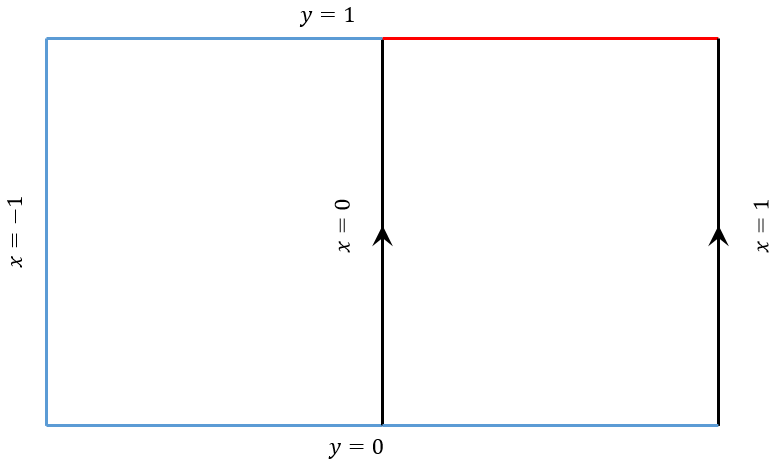
\includegraphics[scale=0.5]{Ex2007imagen1.png} 
		\end{center}
	
	\begin{enumerate}
		\item Para encontrar un subespacio como el que se requieren, basta hallar algún objeto de $\mathbb{R}^3$ en el que se realice una identificación dada por las relaciones de equivalencia anteriormente dadas. El diagrama a seguir es el siguiente
	\[\xymatrix{
S \ar[r] \ar[d]  & X\subset \mathbb{R}^3  \\
S/\sim \ar[ru]^{\sim}_{\mathrm{homeo}}}\]
	Para obtener el conjunto cociente dada por la segunda relación de equivalencia se deberán identificar los puntos $(0,y)$ y $(1,y)$ de cada clase de equivalencia $\{0,1\}\times \{y\}$ a un mismo punto. Como resultado, se obtiene que el conjunto cociente es el cilindro $S^1\times [0,1]$ de $\mathbb{R}^3$ al que se le añade el cuadrado $[-1,0]^2$:
 
		\begin{center}
			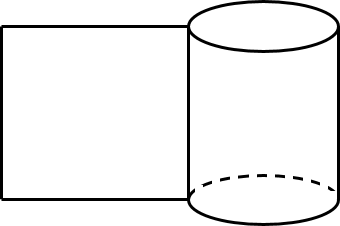
\includegraphics[scale=0.5]{Ex2007imagen2.png} 
		\end{center}
	
	A continuación, la tercera relación de equivalencia viene a decir que todos los puntos que componen la circunferencia superior colapsan en uno, el $(1,0)$:

		\begin{center}
			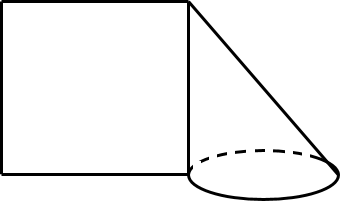
\includegraphics[scale=0.5]{Ex2007imagen3.png} 
		\end{center}
	
	Este esquema es el subconjunto $X$ que buscábamos. Para verlo, basta comprobar que la aplicación $h: S/\sim \to X$ es un homeomorfismo. En resumidas cuentas, al cuadrado $[-1,0]^2$ se le aplicó la identidad y a $[0,1]^2$ una serie de transformaciones continuas. Así, $h$ es una biyección y, por lo que sabemos, continua. No obstante, $S/\sim$ es un conjunto compacto y $X\subset \mathbb{R}^3$ es \hausdorff, luego la aplicación $h$ es un homeomorfismo. Para concluir, cabe destacar que la topología cociente es la topología inducida por $\mathbb{R}^3$.
	
	\item Mostremos que $X$ es simplemente conexo en dos pasos. En primer lugar, hagamos que cualquier punto $p$ del cuadrado $[-1,0]^2$ vaya a $g(p)$ mediante una aplicación $g$ que es continua y tal que $(t,p)\to (1-t)p+tg(p)$ con $t\in[0,1]$. De su definición se deduce que para $t=0$ es la identidad y que para $t=1$ tenemos el punto $g(p)$. De este modo, para un cierto $t$ se ha contraído un poco hacia el cono
	
		\begin{center}
			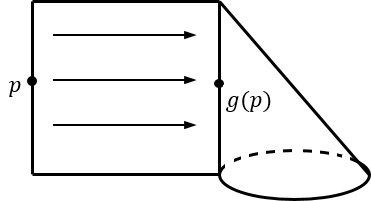
\includegraphics[scale=0.5]{Ex2007imagen4.png} 
		\end{center}
		
	Una vez que únicamente quedan los puntos que el cuadrado compartía con el semicono, se puede hacer algo similar con este último. Si denotamos $c$ al vértice del semicono, la aplicación dada por $(t,p)\to (1-t)p+tc$ con $t\in[0,1]$. 

	Con esto, hemos mostrado que es homeomorfo al punto $c$, luego es simplemente conexo. 
	
	\item Claramente, $X$ no es homeomorfo a una esfera. Para verlo, tomemos el punto $p$ de la figura
		
		\begin{center}
			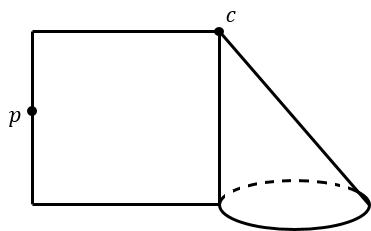
\includegraphics[scale=0.5]{Ex2007imagen5.png} 
		\end{center}
		
	Los entornos del punto $p$ son de la forma
	
		\begin{center}
			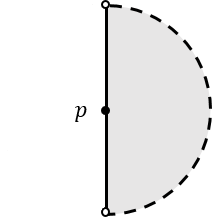
\includegraphics[scale=0.5]{Ex2007imagen6.png} 
		\end{center}
		
que no son homeomorfos a los entornos en cada punto de la esfera (discos abiertos). 
	\end{enumerate}	
\end{proof}

24/04/2017

(1) \emph{Elevación semilocal}. Se trata de una elevación semilocal puesto que solamente se hará localmente en el primer factor del espacio producto $\Y\times [0,1]$. Comprobemos que si fijamos $y\in \Y$ existe una elevación $\tilde{H}^y: V^y\times [0,1]\to \tilde{X}$, donde $V^y$ es un entorno abierto de $y$. Notemos que este entorno puede ser arbitrariamente pequeño. 

En primer lugar, tenemos que $\{y\}\times [0,1]\to X=\cup_x U^x$, donde $U^x$ son los entornos regularmente cubiertos restringidos a $H$. Por ser $\{y\}\times[0,1]$ compacto ($\{y\}$ lo es en $\Y$ y $[0,1]$ en $\X$ respectivamente), existe una partición $0=t_0<t_1<\ldots <t_r$ de modo que $H(\{y\}\times [t_{i-1},t_i])\subset U^{x_i}$, o lo que es lo mismo, $\{y\}\times [t_{i-1},t_i]\subset H^{-1}(U^{x_i})$. No obstante, $H^{-1}(U^{x_i})$ es un abierto de $\Y\times[0,1]$ por ser $H$ continua. 

El lema de Wallace nos dice que existe un entorno $V^y_i$ de forma que $V_i^y\times [t_{i-1},t_i]\subset H^{-1}(U^{x_i})$. Por consiguiene , podemos considerar
\[V^y=\bigcap_{1\leq j\leq r}V_j^y,\]
entorno abierto  (por ser intersección finita de abiertos) de $y$, luego 
\[V^y\times[t_{i-1},t_i]\subset H^{-1}(U^{x_i})\]
y es posible definir correctamente $H: V^y\times [t_{i-1},t_i]\to U^{x_i}$ para todo $i\in\{1,\ldots, r\}$. 

Por inducción, elevamos esta restricción de $H$ (recordemos que queremos elevar todo el intervalo $[0,1]$). Sabemos que $\tilde{H}^y |_{V^y\times \{0\}}=\tilde{H}_0^y=\tilde{f}$. Supongamos que la elevación $\tilde{H}^y |_{V^y\times [0,t_i]}$ está definida. Para poder definir correctamente la elevación en $[t_i,t_{i+1}]$, ambas han de coincidir en $t_i$. Tal y como hemos tomado $V^y$ en el razonamiento anterior, podemos tomar $H:V^y\times[t_i,t_{i+1}]\to U^{x_{i+1}}$ y, por consiguiente, $H(y,t_i)\in U^{x_{i+1}}$. 

Por un lado, se tiene que la elevación $\tilde{H}^y|_{V^y\times[0,t_i]}$ está definida en el punto $(y,t_i)$, luego al ser 
\[p(\tilde{H}^y|_{V^y\times [0,t_i]}(y,t_i))=H(y,t_i)\in U^{x_{i+1}},\]
entonces
\[\tilde{H}^y|_{V^y\times [0,t_i]}(y,t_i)\in p^{-1}(U^{x_{i+1}})=\bigcup_\lambda U_\lambda^{x_{i+1}}.\]
Pero al ser $U^{x_{i+1}}_\lambda$ disjuntos, existe un único $\lambda$ tal que $\tilde{H}|_{V^y\times[0,t_i]}(y,t_i)\in U_{\lambda}^{x_i+1}$, o equivalentemente, $(y,t_i)\in (\tilde{H}|_{V^y\times[0,t_i]})^{-1}(U_{\lambda}^{x_i+1})$. Ahora, al ser la elevación continua y $U_{\lambda}^{x_i+1}$ un abierto, la imagen inversa es un abierto del producto $V^y\times [0,t_i]$, de modo que existe un entorno abierto $W^y\subset V^y\subset \Y$ tal que $W^y\times\{t_i\} \subset (\tilde{H}^y|_{V^y\times [0,t_i]})^{-1}(U_\lambda^{x_{i+1}})$. Como ya adelantamos al principio, se puede reducir $V^y$ de modo que su intersección con $W^y$ sea él mismo, por lo que también se cumple que $V^y\times\{t_i\} \subset (\tilde{H}^y|_{V^y\times [0,t_i]})^{-1}(U_\lambda^{x_{i+1}})$. 

A continuación, al ser $p|_{U_\lambda^{x_{i+1}}}$ un homeomorfismo, podemos hacer la siguiente construcción
		\[\xymatrix{
V^y\times[t_{i-1},t_i] \ar[r]^-H \ar[rd] &
U^{x_i} \ar[d]^{p|_{U_{\lambda}^{x_{i+1}}}} \\
&U_{\lambda}^{x_i}}\]
Con ella, vemos que $\tilde{H}|_{V^y\times [t_i,t_{i+1}]}=(p|_{U_{\lambda}^{x_{i+1}}})^{-1}\circ H$. Para ver que está bien definida es necesario que ambas aplicaciones coinciden en $V^y\times \{t_i\}$. Por un lado, al ser
\[(\tilde{H}^y|_{V^y\times [0,t_i]})(V^y\times\{t_i\}) \subset U_\lambda^{x_{i+1}},\]
se tiene que $V^y\times [0,t_i]$ es una elevación de $V^y\times\{t_i\}$ a $U_\lambda^{x_{i+1}}$, y lo mismo ocurre con $\tilde{H}^y|_{V^y\times [t_i,t_{i+1}]}$. De este modo, dado $(y,t_i)\in V^y\times\{t_i\}$ se tiene que 
\[p|_{U_{\lambda}^x}(\tilde{H}^y|_{[0,t_{i}]}(y,t_i))=H(y,t_i)=p|{U_{\lambda}^x}(\tilde{H}^y|_{[t_i,t_{i+1}]}(y,t_i)).\]
Como $p|_{U_{\lambda}^{x_{i+1}}}$ es un homeomorfismo, para todo $(y,t_i)\in V^y\times\{t_i\}$ se tiene que 
\[\tilde{H}^y|_{[0,t_{i}]}(y,t_i)=\tilde{H}^y|_{[t_i,t_{i+1}]}(y,t_i).\]
Con esto, se concluye que
\[ \tilde{H}^y|_{V^y\times [0,t_{i}]} = \begin{cases}
\tilde{H}^y|_{V^y\times [0,t_{i}]} & \text{ si } 0\leq t \leq t_i \\
\tilde{H}^y|_{V^y\times [t_i,t_{i+1}]} & \text{ si } t_i\leq t \leq t_{i+1}
\end{cases}\]
es continua y está bien definida. 

\emph{Pegado}. Por último, hemos de comprobar que las elevaciones $\tilde{H}^y:V^y\times[0,1]\to \tilde{\X}$ son compatibles. Para ello, dadas dos elevaciones $\tilde{H}^y:V^y\times[0,1]\to \tilde{\X}$ y $\tilde{H}^{y'}:V^{y'}\times[0,1]\to \tilde{\X}$, hemos de comprobar que coinciden en $(V^y\cap V^{y'})\times[0,1]$. Así, la aplicación global estará bien definida desde el punto de vista conjuntista. 

En efecto, consideremos $y''\in V^y\cap V^{y'}$ y veamos que 
\[\tilde{H}^y(y'',\bullet)=\tilde{H}^{y'}(y'',\bullet).\]
No obstante, al ser dos elevaciones de $H$ en $\{y''\}\times[0,1]$, se tiene que 
\[\tilde{H}^y(y'',0)=\tilde{H}^{y'}(y'',0)=\tilde{f}(y'').\]
Al tenerse dos elevaciones en un conexo ($\{y''\}\times[0,1]$) que coinciden en un punto, entones por unicidad son iguales. 
\end{itemize}